%Please use LuaLaTeX or XeLaTeX
\documentclass[11pt,aspectratio=169]{beamer}

\title{Theta Functions, Kronecker Functions, and Bilinear Relations}
\date[2023]{Riemann Surfaces \\ in Mathematical Physics}
\author{Artyom Lisitsyn}
\institute{D-PHYS}

\usetheme{eth}

\colorlet{titlefgcolor}{ETHBlue}
\colorlet{accentcolor}{ETHRed}

\usepackage{cancel}

\begin{filecontents}{\jobname.bib}
    @book{Ber06,
        Author = {Marco Bertola},
        Title = {Riemann Surfaces and Theta Functions},
        Year = {2006}}

    @article{Cha22,
        Author = {Zhi Cong Chan},
        Title = {Towards a Higher-Genus Generalization of the
        Kronecker Function Using Schottky Covers},
        Year = {2022}
    }
\end{filecontents}
\usepackage[backend=bibtex,style=authoryear, defernumbers=true]{biblatex}
\addbibresource{\jobname.bib}
\begin{document}

% Find better title image?
\def\titlefigure{elements/title-page-image}
\titleframe{}

\tocframe{}

\section{Abel's map}

\begin{frame}{Holomorphic Differentials}
    \begin{block}{Existence of holomorphic differentials}
        The dimension of the space of holomorphic differentials is $\dim \mathcal H^1 = g$, the genus of the compact Riemann surface.
    \end{block}

    \begin{columns}[onlytextwidth]
        \begin{column}{0.55\textwidth}
            \emph{Proof outline:}
            \begin{itemize}
                \item $\dim \mathcal H^1 \leq \text{\# of a-cycles} = g$
                \item $\text{\# of harmonic differentials} = \dim H \geq 2g$
                \item $h = f dz + g d \bar z \implies \dim H = 2 \dim \mathcal H^1$
                \item $g \leq \dim \mathcal H^1 \leq g \implies \dim \mathcal H^1 = g$
            \end{itemize}
            \emph{Normalization \& period matrix:}
            \[ \int_{a_i} \omega_j = \delta_{ij} \]
            \[ \int_{b_i} \omega_j = \tau_{ij} \]
        \end{column}
        \begin{column}{0.45\textwidth}
            \center{}
            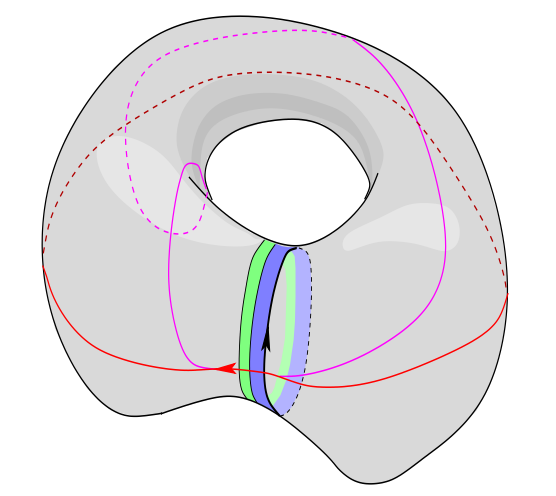
\includegraphics[width=0.8\columnwidth]{assets/HarmonicDifferential.png}
            
            \tiny Regions used to define harmonic differentials

            \cite{Ber06}
        \end{column}
    \end{columns}
\end{frame}

\begin{frame}{Abel's map}
    \begin{block}{Formal definition of Abel's map}
        For a particular choice of a point $P_0$ on the fundamental domain $\mathcal L$, using the normalized harmonic differentials $\omega_i$, we have Abel's map
        \begin{align*}
            \mathbf{u} : \mathcal L & \mapsto \mathbb{C}^g & \\
            P & \mapsto \begin{pmatrix} \int_{P_0}^P \omega_1 \\ \vdots \\ \int_{P_0}^P \omega_g \end{pmatrix} &
        \end{align*}
    \end{block}

    \emph{Analytic continuation beyond the fundamental domain:}
    \[\mathbf{u}(P+a_i) = \mathbf{u}(P) + \begin{pmatrix} \int_{a_i} \omega_1 \\ \vdots \end{pmatrix} = \mathbf{u}(P) + \begin{pmatrix} \delta_{i1} \\ \vdots \end{pmatrix}\]
    \[\mathbf{u}(P+b_i) = \mathbf{u}(P) + \begin{pmatrix} \tau_{i1} \\ \vdots \end{pmatrix}\]
\end{frame}

\begin{frame}{Abel's map at genus 1}
    \begin{columns}[onlytextwidth]
        \begin{column}{0.55\textwidth}
            Appropriate differential
            \[\omega = dz\]
            
            Abel's map
            \[\mathbf{u}(z) = \int_0^z \omega = z\]
        \end{column}
        \begin{column}{0.45\textwidth}
            \center{}
            \includegraphics[width=0.7\columnwidth]{example-image-a}

            \tiny Fundamental domain and continuation at genus 1

            \cite{ImageSource}
        \end{column}
    \end{columns}

    {
    % \setbeamercolor{block body}
    \setbeamercolor{block title}{bg=ETHBlue}
    \setbeamercolor{block body}{bg=ETHBlue!25!white}
    \begin{block}{What about higher genus?}
        \begin{itemize}
            \item How do we represent the fundamental domain?
            \item What choice of differentials can we make?
            \item What consequences does this have for Abel's map?
        \end{itemize}
    \end{block}
    }
\end{frame}

\section{Theta functions}

\begin{frame}{Theta functions}
    \begin{block}{Definition of the Theta function}
        Given a symmetric matrix $\tau$ with positive definite imaginary part, the Theta function is
        \[\Theta(\vec z, \tau) := \sum_{\vec n \in \mathbb Z^g} \exp \left(2 \pi i \left[ \frac{1}{2} \vec n^T \tau \vec n + \vec n^T \vec z \right]\right)\]
    \end{block}

    \emph{Properties:} For $\vec \lambda \in \mathbb Z^g$

    \[\Theta(-\vec z) \overset{\vec n \mapsto -\vec n}{=} \Theta(\vec z)\]

    \[\Theta(\vec z + \vec \lambda) = \sum_{\vec n \in \mathbb Z^g} \cancelto{1}{\exp(2\pi i \vec n^T \vec \lambda)} \exp(\ldots) = \Theta(\vec z)\]

    \[\Theta(\vec z + \tau \vec \lambda) = \begin{bmatrix} \text{shift } \vec n \\ \text{use }\tau\text{ symmetry}\end{bmatrix} = \exp\left(2\pi i\left[- \frac{1}{2}\vec \lambda^T \tau \lambda-\vec \lambda^T \vec z\right]\right)\Theta(\vec z)\]
\end{frame}

\begin{frame}{Theta function on a compact Riemann surface}
    \begin{block}{Definition of Theta function on a compact Riemann surface}
        For a compact Riemann surface $\mathcal M$ of genus $g$, with period matrix $\tau$ and Abel's map $\mathbf{u}$, we can identify
        \begin{align*}
            \theta : \ & \mathcal M \mapsto \mathbb C \\
            & P \mapsto \Theta(\mathbf{u}(P))
        \end{align*}
    \end{block}

    \emph{Properties:}
    \[ \theta(P + a_i) = \theta(P) \]

    \[ \theta(P + b_i) = \exp\left(2\pi i\left[- \frac{1}{2} \tau_{ii} - \mathbf{u}_i(P) \right]\right)\theta(P) \]
\end{frame}

\begin{frame}{Theta function at genus 1}
    \begin{columns}[onlytextwidth]
        \begin{column}{0.55\textwidth}
            \[\theta(z) = \sum_{n \in \mathbb Z} \exp(2\pi i[\frac{1}{2}n^2 \tau + n z])\]

            \[\theta(z)=\theta(-z)\]
            \[\theta(z+1)=\theta(z)\]
            \[\theta(z+\tau)=\theta(z)\]
        \end{column}
        \begin{column}{0.45\textwidth}
            \center{}
            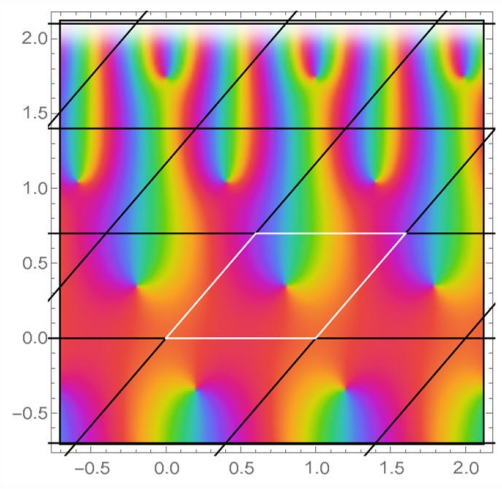
\includegraphics[width=0.7\columnwidth]{assets/genus1theta.png}

            \tiny Theta function for $\tau = 0.7+0.6i$
            
            \cite{Cha22}
        \end{column}
    \end{columns}

    {
    % \setbeamercolor{block body}
    \setbeamercolor{block title}{bg=ETHBlue}
    \setbeamercolor{block body}{bg=ETHBlue!25!white}
    \begin{block}{What about higher genus?}
        \begin{itemize}
            \item What does the Theta function look like at higher genus?
        \end{itemize}
    \end{block}
    }
\end{frame}

\begin{frame}{(Application) Decomposing meromorphic functions and differentials}
    Rough outline of how to reproduce a function with divisor $(f) = \sum n_i P_i$
    \[ \begin{bmatrix}\text{Find function }t(z) \\ \text{such that }t(0)=0\end{bmatrix} \rightarrow \begin{bmatrix} g(z)=\prod t(P-P_i)^{n_i} \\ \text{respecting possible periodicity}\end{bmatrix} \rightarrow \left(\frac{f}{g}\right) = \emptyset \rightarrow \frac{f}{g} = \text{const.} \]
    \begin{columns}
        \begin{column}{0.5\textwidth}
            At Genus 0:
        \end{column}
    \end{columns}
\end{frame}

\section{Kronecker function}

\begin{frame}
    kronecker
\end{frame}

\section{Striving for higher genus}

\begin{frame}
    motivation
\end{frame}

\begin{frame}{References}
    \printbibliography{}
\end{frame}

\end{document}